\documentclass{article}
\usepackage[utf8]{inputenc}
\usepackage{indentfirst}
\usepackage{amsmath}    % load AMS-Math package
\usepackage{epsfig}     % allows PostScript files
\usepackage{listings}   % allows lstlisting environment
\usepackage{moreverb}   % allows listinginput environment
\usepackage{vmargin}    % allows better margins
\setpapersize{USletter} % sets the paper size
\usepackage{graphicx}
\usepackage{mathrsfs}
\usepackage{diagbox}
\usepackage{lettrine}
\usepackage{tabto}
\setmarginsrb{1in}{0.5in}{1in}{0.2in}{12pt}{11mm}{0pt}{11mm} %sets margins 


\begin{document}
\title{ECE 350: Digital Systems Project Checkpoint 4}
\author{Siyuan Chen} % Change this to your name
\date{\today} % Change this to the date you are submitting
\maketitle

\section*{Duke Community Standard}

By submitting this \LaTeX{} document, I affirm that
\begin{enumerate}
    \item I understand that each \texttt{git} commit I create in this repository is a submission
    \item I affirm that each submission complies with the Duke Community Standard and the guidelines set forth for this assignment
    \item I further acknowledge that any content not included in this commit under the version control system cannot be considered as a part of my submission.
    \item Finally, I understand that a submission is considered submitted when it has been pushed to the server.
\end{enumerate}

\section{Introduction}
This document serves as a comprehensive description of the ECE 350 processor. The ECE 350 processor is a single-issue, in-order pipelined processor that executes the ECE 350 ISA (found in Appendix A) and the pipeline contains five stages: Fetch, Decode, Execute, Memory and Writeback. The rest of this document discusses in detail the design and implementation of this processor.

\section{Subcomponents}
\subsection{Regfile}
\subsubsection{Design}
The register file contains 32 registers. Each register is 32-bit and uses positive-edge-triggered D-Flip-Flops with write-enable as basic memory elements. The register file has two read ports and one write port. The read ports select data with tri-state buffers. It needs to be clocked on the positive edge to avoid data hazards. 
\subsubsection{Special Registers}
\texttt{\$r0} is always zero. \texttt{\$r30}, also called \texttt{\$rstatus}, is set to a non-zero value (more details in Section 4) when an exception occurs. \texttt{\$r31} or \texttt{\$ra} is the return address register.

\subsection{ALU}
The 32-bit ALU is the main execution unit. It supports addition, subtraction, bitwise and, bitwise or, logical left shift and arithmetic right shifts. Addition and subtraction are implemented with a hybrid carry-select-carry-lookahead adder, while shift operations are implemented with barrel shifters. \par
During an addition or subtraction execution, overflow is detected and outputted as a flag signal that could be captured by higher level components. During subtraction, the ALU also outputs two flags: \texttt{isNotEqual} and \texttt{isLessThan}, which are used in conditional branches.

\subsection{MultDiv}
The 32-bit Multdiv unit executes multiplication and division instructions. The modified-booth multiplier takes 17 cycles to output a correct result while the divider takes 34 cycles. When the result is ready, the \texttt{data\_resultRDY} flag will be set to one. At the same time, an exception flag that detects overflow in multiplication and division-by-zero in division will be outputted. 

\subsection{Memory}
The memory system of the ECE 350 processor consists of two parts: instruction memory (imem) and data memory (dmem). Both of them are implemented using the \texttt{altsynchram} megafunction in Altera Quartus. Both of them are 12-bit addressed and the word size is 32 bits. The instruction memory has only a single read port while the data memory has one read port and one write port.

\section{Full Processor}
\subsection{Design implementation details of each stage}
\subsubsection{Fetch}
In the Fetch stage, the current instruction is read from the imem using the current program counter (PC). An adder increments PC by one. Then, branch signal computed in the Execute stage selects if the next PC is a branch target or PC+1.

\subsubsection{Decode}
In the Decode stage, in the first half of a cycle, Writeback stage writes the newly computed result into the register file. In the second half of the cycle, the current values of the to-be-read registers are read. Since not all instructions take \texttt{\$rs, \$rt} as their first and second register to read, logic is implemented to select the correct register index. \par
In addition, considering that the ALU will take a very large portion of the clock period in Execute stage, I decided to put some of the select logic for ALUinB into the Decode stage, and then pass these signals to the next stage through a D-Flip-Flop so that the ALU could directly start executing in the Execute stage without the need to wait for selecting logic to complete.

\subsubsection{Execute}
In the Execute stage, the ALU or the MultDiv unit executes arithmetic computation. The details about stall and bypass logic in the Execute stage in the section 3.2 and 3.3. \par
At the same time, branches resolve in the Execute stage. By branches, the author refers to all the instructions that could result in a change in PC. The details about each instruction will be discussed in Section 4.

\subsubsection{Memory}
In the Memory stage, the instruction, if it is a \texttt{lw} or \texttt{sw}, accesses the dmem to read from/write to data memory. In addition, results from the previous Execute stage is bypassed to the current Execute stage if needed.

\subsubsection{Writeback}
In the Writeback stage, the instruction writes its value back to the \texttt{\$rd} register. In addition, the writeback data is bypassed to the current Execute stage if needed; if the current instruction in the Memory stage is a \texttt{sw} whose value depends on the writeback value, this value is also bypassed to the Memory stage.

\subsection{Handling Hazards}
The ECE 350 processor integrates stalling, flush logic and full bypassing to avoid hazards while maintain high performance. Since the pipeline is issuing in-order, only RAW data hazards need to be considered. This section mainly discusses stalling while the next section will focus on bypassing. \par
With full bypassing implemented, there are only two situations where the processor needs to stall:
\begin{itemize}
    \item When a load instruction is followed immediately by an instruction that depends on the load (except when the dependent instruction is a store that needs the value from the load), the processor stalls for a cycle. When stalling, PC register and instruction register between fetch and decode is set to not-writable. A noop is inserted into the execute stage.
    \item When there is a multdiv operation, the processor stalls until the dataRDY flag in the MultDiv unit is one. During multdiv stalls, the X/M registers hold their values so that the result could be written once the multdiv finish computing.
\end{itemize}

\subsection{Bypassing Logic}
The ECE 350 processor implements full bypassing: WX, MX and WM. The general logic is: whenever an instruction in Writeback or Memory writes to a register that instructions in Execute or Memory need, this data is bypassed. This logic is implemented using combinational circuits and MX, WX bypassed data is selected using multiplexers in Execute stage.

\subsection{Processor Clock}
With a 50 MHz clock, the processor would expect to have full functionality. If the clock gets faster beyond this threshold, some arithmetic functions such as subtraction is likely to produce intermediate wrong results.

\subsection{Efficiency Detail}
Efficiency of the ECE 350 processor comes in the following ways:
\begin{itemize}
    \item Full bypassing is implemented.
    \item Branches resolve in the Execute stage.
\end{itemize} \par
To further improve efficiency, the author proposes several ways:
\begin{itemize}
    \item Add a branch predictor in Fetch stage.
    \item Pipeline MultDiv unit, or even more aggressively, execute non-dependent instructions but stay in-order.
\end{itemize}

\section{Instruction Implementation}
\subsection{Arithmetic Instructions}
Arithmetic instructions read their register values in the Decode stage, and are executed either by the ALU or the MultDiv. The two inputs in these units are selected with bypassed values and the result is passed to Memory stage and finally written back in Writeback stage. When they produce overflows and exceptions, the instruction is changed into the specific \texttt{setx} instruction and passed to the Memory stage. Since the value is wrong, writing it back is not necessary.

\subsection{Memory Instructions}
For memory instructions, the address in computed in the Execute stage through the ALU (register input could be bypassed). Then the address is used to write/read the data in the Memory stage. \texttt{sw} may need the WM bypassing data.

\subsection{Branch Instructions}
\subsubsection{blt, bne, bex}
These conditional branches use the isLessThan and isNotEqual flag produced by the ALU to determine if the PC will be changed. A separate adder is used to compute the branch target. It is selected in a multiplexer with possible jump or jr targets.

\subsubsection{j, jr, jal}
For these unconditional jumps, their target is sign extended and selected in the same multiplexer mentioned above. jal will propagate to the Writeback stage in which there is special logic to write the value back to \texttt{\$ra}.

\subsection{setx}
In the writeback stage, there is separate logic for checking setx. Correspondingly, the index of the write register will be set to \texttt{\$r30} if the instruction is a setx and the data written back set as the sign extended immediate.

\section{Process}
\subsection{Choice of Implementation}
The main reason I chose my implementation is that it is the most intuitive and familiar one for me. In addition, I implemented full bypassing because I understood how much it could boost performance. The two big design choices I had to make are:
\begin{itemize}
    \item How to add the MultDiv: although I know there are more efficient ways, I chose to stall the processor when a multdiv instruction is running.
    \item I chose to change the instruction to a setx when an exception occurs for an arithmetic instruction in case of complexity considerations: the processor do not need separate logics between setx and arithmetic exceptions.
\end{itemize}

\subsection{Test of Implementation}
I wrote several assembly code snippets that test every instructions, control logic, data hazards and exception. Then I ran these sample programs with a testbench outputting important information such as writeback data and register, ALU inputs and outputs to verify them.

\subsection{Remaining Issues}
The exception signal of multiply and divide would not be caught at this point. According to the design of multdiv mentioned above, when this overflow occurs, the X/M registers would not be writable (as at this point instructions in execute stage are noops) and therefore more logic need to be added so that these overflow values could be latched properly in order to propagate to writeback.

\subsection{Challenges}
One of the main challenges I faced is implementing the bypassing logic. This logic is very complicated and easy to make mistakes. After a first implementation, I spent a whole day debugging bypassing, thinking of test cases and finding the logic errors.

\subsection{Learning points}
I think the main learning point from this project is the whole engineering process: building, testing, finding bugs and trying to solve them. I feel like an electrical engineer after this project.

\section{Conclusion}
The ECE 350 processor is a single-issue, in-order processor with a 5-stage pipeline. It runs the ECE 350 ISA and is optimized with full bypassing and flush logics.

\newpage
\appendix
\section{ISA}
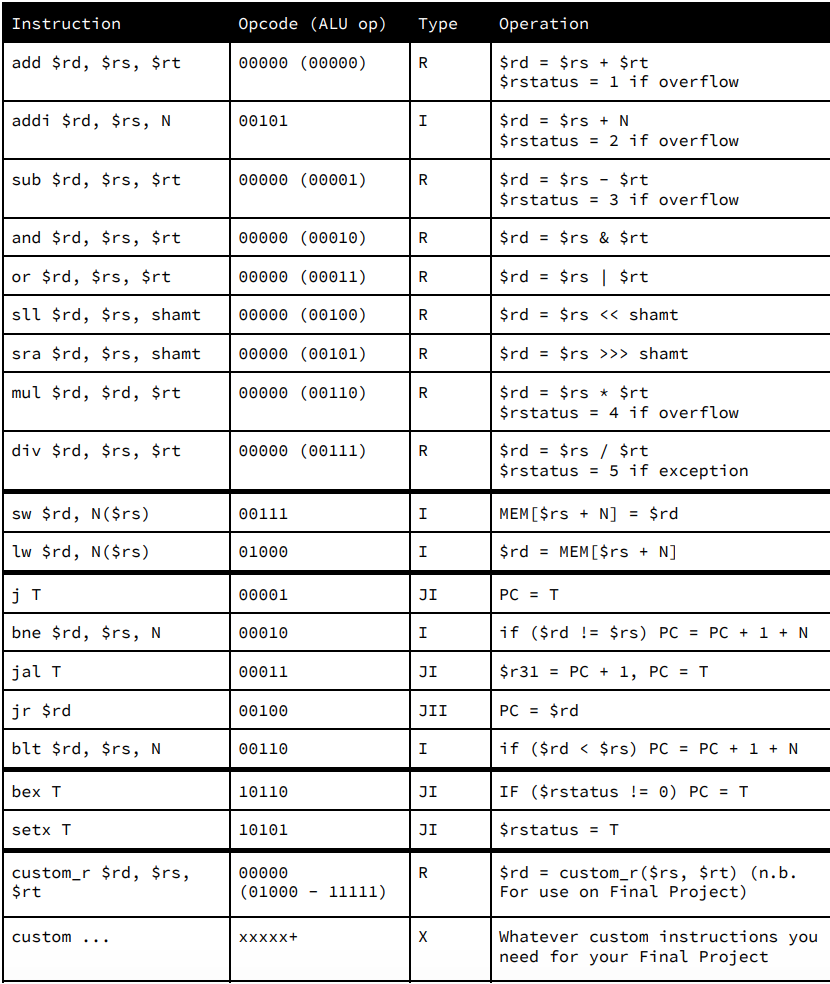
\includegraphics[width=\textwidth]{image/ISA.png}
\end{document}
